\section{Generate Test Cases}
\marginnote{Most books talk about correct solutions only.  Few books
  talk about incorrect methods and why they are wrong.  This book
  takes a different approach: we assume that mistakes are unavoidable
  and explain strategies to prevent, detect, and correct the mistakes.
}

Lacking test cases of known properties is one common problem in
developing software for machine learning.  The purpose of machine
learning is to recognize unknown patterns in data; thus, we do not
know the patterns in advance.  How can we know that the programs are
correct?  If we do not know that the programs are correct, how do we
know the patterns discovered by the programs are correct?  Two methods
are commonly used:
\begin{enumerate}
\item Creating simple test cases manually with known properties.

\item Adopting widely used test cases whose properties have already
  been studied.
\end{enumerate}
The first methods is restricted to only very small test cases that are
unlikely to have sophisticated patterns needed to test computer
programs.  The second methods, in contrast, may sophisticated patterns
but the data may be too complex for identify problems in the programs.

\index{test case generator}

\marginnote{When developing programs, it is common to test using cases
  of known properties generated by computer programs (called {\it test
    case generators} in this book).  }

This book suggests the third approach: write another program (or
several programs) to generate the test cases of known properties.
More specifically, for this problem, we can write a program that
generates $n$ data points in $k$ clusters ($n > k$).  Since the data
points are generated intentionally, it is easy to test whether a
k-mean program is correct.

Writing a test case generator, however, is not trivial because the
generator has to consider many different possible properties of data
collected in different scenarios. It is likely that different
generators would be needed in different scenarios. This section
explains one generator. Readers may need to change this generator to
meet different needs.  This generator has the following input
arguments:\marginnote{Determining the inputs is an important part of
  designing software.}

\begin{itemize}
\item Number of dimension ($p$ in the explanation).  Each data point
  is a $p$-dimensional vector. The minimum value is 1.

\item Number of clusters (called $m$ in this program).  This program
  restricts that $m$ must be greater than two.  The program
  intentionally uses a different symbol ($m$) to distinguish from the
  value $k$ given to the clustering program to be tested.

\item Minimum numbers of data points per cluster (called $q$ in this
  program).  This program restricts that $q$ must be at least three.

\item Maximum numbers of data points per cluster (called $r$ in this
  program). Obviously, $r$ must be greater than $q$.

\end{itemize}  

All these arguments are positive integers.  The programs in this
chapter handles integers only because floating-point numbers have
limited precision and sometimes give suprising results.  The number of
data points $n$ is between $m q$ and $m r$.
\marginnote{Chapter~\ref{ch:floatingpoint} has more details about how
  the limited precision may affect results in analysis.}  This program
generates two output files: {\tt data.txt} and {\tt cluster.txt}.  The
first file has $n$ lines and each line has $p$ integers.  The second
file also has $n$ lines; each line has the same $p$ integers,
following by one integer between $0$ and $m - 1$ to indicate which
cluster this line belongs to.

This program is pretty simple: it divides $(-1000m, 1000m)$ in each
dimension into $m$ regions. The centroids of two adjacent regions are
separated by 2000 in each dimension.  The data points of a particular
cluster are scattered within 200 around the cluster's centroid.  The
following is the test case generator.

\resetlinenumber[1]
\linenumbers
\begin{tt}
  \lstinputlisting{\progpath/unsupervised/kmean/testgen/main.py}
\end{tt}
\nolinenumbers

\resetlinenumber[1]
\linenumbers
\begin{tt}
  \lstinputlisting{\progpath/unsupervised/kmean/testgen/testgen.py}
\end{tt}
\nolinenumbers

This is a sample output of the program using the default values for
the arguments: $(p, m, q, r) = (2, 3, 3, 5)$.
This is an example of the output {\tt data.txt}.

\resetlinenumber[1]
\linenumbers
\begin{tt}
  \lstinputlisting{\kmeanpath/data/data.txt}
\end{tt}
\nolinenumbers

This is an example of the corresponding {\tt cluster.txt}.

\resetlinenumber[1]
\linenumbers
\begin{tt}
  \lstinputlisting{\kmeanpath/data/cluster.txt}
\end{tt}
\nolinenumbers

\section{Visualize Data}

\index{high-dimensional}

This chapter presents a program that can visualize data up to three
dimensions.  The purpose of this visualization is to help inspect
whether the data produced by the test generator is indeeded clustered
into several regions.

\resetlinenumber[1]
\linenumbers
\begin{tt}
  \lstinputlisting{\progpath/unsupervised/kmean/testgen/visualize.py}
\end{tt}
\nolinenumbers

\marginnote{It is common that the data of interest is {\it
    high-dimensional} and visualizing the data would be difficult.  }

The following figures show the generated data in one, two, and three
dimensions.  The figures are drawn using {\tt visualize.py}.


\clearpage

\begin{figure}[h] \centering
 \subfigure[]
{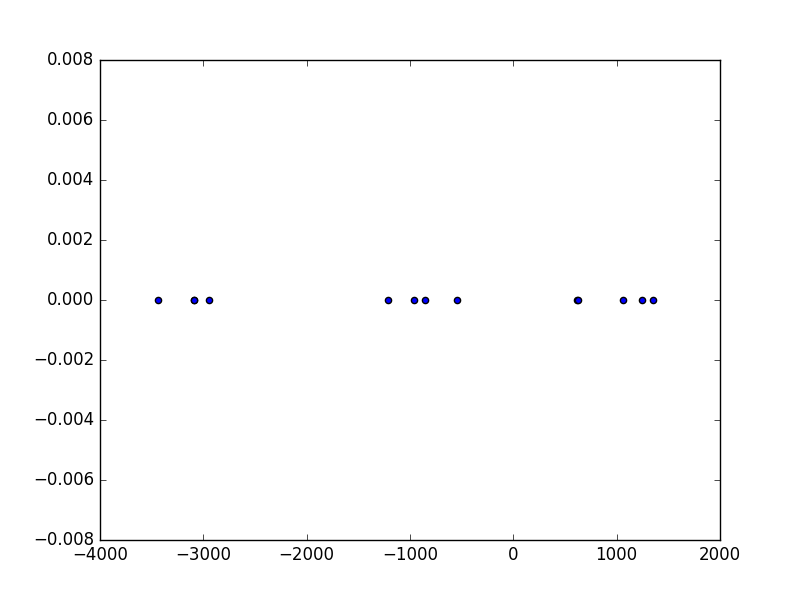
\includegraphics[width=3in]{\kmeanpath/figures/figure1.png}}
  \subfigure[]
{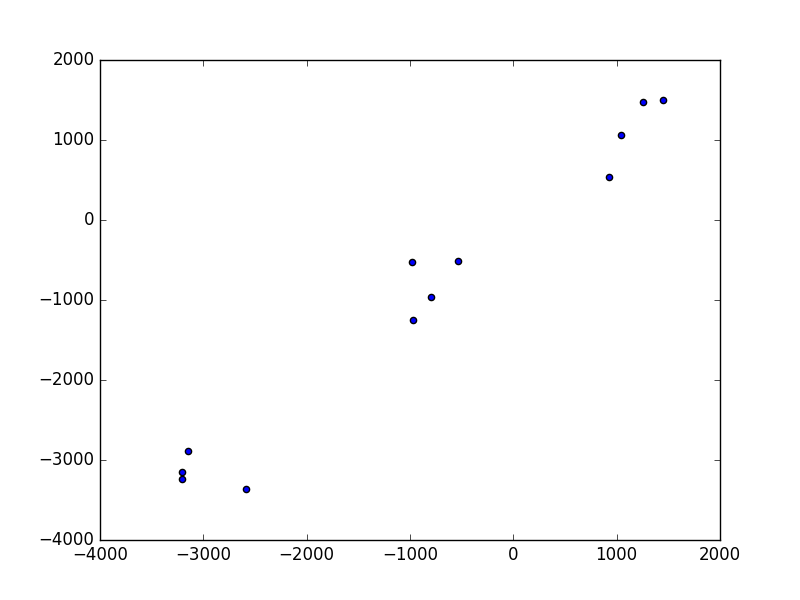
\includegraphics[width=3in]{\kmeanpath/figures/figure2.png}}
  \subfigure[]
{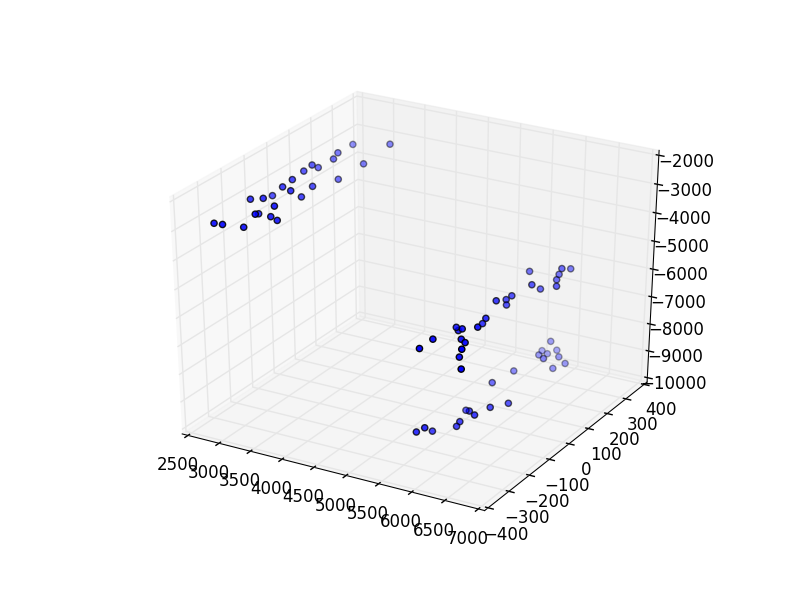
\includegraphics[width=3in]{\kmeanpath/figures/figure3.png}}
\caption{Visualize the generated test cases in one, two, and, three
  Dimensions. }
\label{fig:kmean:visualize}
\end{figure}

\clearpage

\section{K-Mean Algorithm Implementation}

Now is the time to show how the {\it K-Mean} algorithm
can be implemented.

Chapter~\ref{ch:clusterlimit}
will explain some other factors for consideration.
